\section{Capabilities Approach}
\label{equity-sec:sen-ca}

Following the discussion, the \glsfirst{CA} was proposed by Amartya Sen and puts the focus on other aspects when analyzing equity issues. Sen is an Indian economist and philosopher who follows the liberal tradition (like Rawls). He is known for his contributions to the creation of the \gls{HDI} \cite{bomfim:2012} and for winning the Nobel Prize \cite{nobel:2022}.

The main question raised by \citeonline[p.~12]{sen:1992} is "equality of what?". Sen's concerns concentrated on the higher risk of reducing the efforts to deal with inequalities to a single-dimensional analysis. The inequality problem is complex and multidimensional by nature. Thus, when we analyze the problem only with the incoming inequality lens, for instance, other sources of inequalities can probably be neglected and, in some cases, even aggravated. Although the race lens, for example, can contribute to informing essential aspects that can not be overlooked by all stakeholders responsible for analyzing a given scenario, this one is not enough to inform a decision-maker with quality and robustness if isolated from others.

The unifier key point for Sen is the freedom to achieve well-being. Well-being is an issue of primary moral importance in Sen's perspective. The well-being prism is the umbrella that allows for a more diverse analysis from different sources of inequities to dialog to achieve a single (but complex) commitment. In summary, the first normative claim of the theoretical framework of the \gls{CA} is that the freedom to achieve well-being is of primary moral importance. \citeonline[p.~3]{dreze:2002} explore this direction, asserting that:
\begin{citacao}
    "It should be clear that we have tended to judge development by the expansion of substantive freedoms - not just by the economic growth (for example, of the gross national product), or technical progress, or social modernization. This is not to deny, in any way, that advances in the latter fields can be very important, depending on circumstances, as ''instruments'' for the enhancement of human freedom. But they have to be appraised precisely in that light - in terms of their actual effectiveness in enriching the lives and liberties of people - rather than taking them to be valuable in themselves".
\end{citacao}

The second \gls{CA} claim is that the understanding of well-being is directly related to people's capabilities and functionings. When Sen attaches the proper comprehension of well-being to the concepts of functioning (Section \ref{sen-ss:functioning}) and capability (Section \ref{sen-ss:capability}), he shifts the concern to defining what well-being is exactly, exploring these two crucial \gls{CA} concepts in more detail. Honestly, Sen's contribution resides primarily in this shifting, indicating the primacy of well-being but does not exhaust it. Sen allows a certain plasticity level of his approach not to define well-being categorically. However, he establishes three concepts for guiding the discernment of dealing with an analysis from a multidimensional inequity perspective. Beyond functionings and capabilities, conversion factors (Section \ref{sen-ss:conv-fac}) are the third essential \gls{CA} concept.

\subsection{Functioning}
\label{sen-ss:functioning}

As mentioned, Sen does not define well-being but characterizes it in terms of functionings and capabilities. About functionings, he asserts that:
\begin{citacao}
    "The well-being of a person can be seen in terms of the quality of the person's being. Living may be seen as consisting of a set of interrelated ''functionings'', consisting of beings and doings. A person's' achievement in this respect can be seen as the vector of his or her functionings. The relevant functionings can vary from such elementary things as being adequately nourished, being in good health, avoiding escapable morbidity and premature mortality, etc., to more complex achievements such as being happy, having self-respect, taking part in the life of the community, and so on" \cite[p.~39]{sen:1992}.
\end{citacao}
Thus, functionings are beings and doings that are "various states of human beings and activities that a person has achieved" \cite{robeyns:2023}.

From an educational perspective, I can exemplify this concept from a political-pedagogical project of a computing program. When a professor's group delineates a graduate profile, it idealizes all the expected functionings that a student should achieve after the completion of the course. In this way, beings like "to be proactive" or "able to work in groups", and doings like "sorting an array" and "modeling a database" are functioning descriptions. All these would be relevant functionings that a graduate should have. Thus, there is a vector of interrelated functionings that describes a graduate profile appropriately (see Figure \ref{fig:graduate-profile}).

\begin{figure}[ht!]
    \centering
    
    \caption{\textmd{Schema of a Computer Science graduate profile composed by beings and doings.}}
    \label{fig:graduate-profile}
    \fcolorbox{gray}{white}{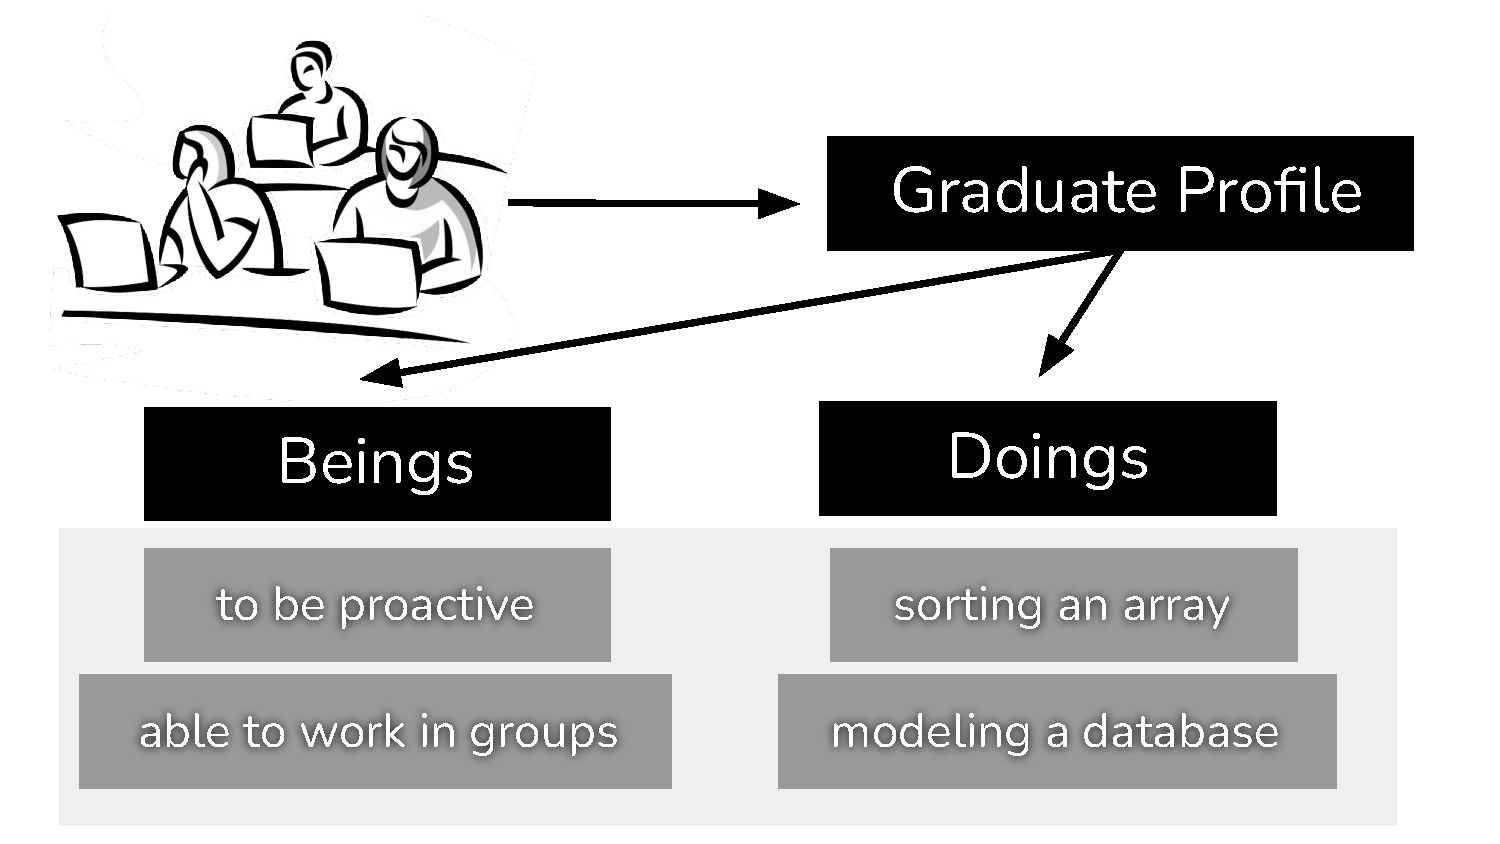
\includegraphics[width=0.9\textwidth]{images/chapter-03/graduate-profile.pdf}}
    
    \par\medskip\ABNTEXfontereduzida\selectfont\textbf{Source:} Created by the author (2024). \par\medskip
\end{figure}

A concrete example can be extracted from the \gls{CC2020} proposed by a task force conducted by \gls{ACM} and \gls{IEEE-CS}. The \gls{CC2020} \cite[p.~52]{acm:2020} embraced competency lens for all its computing curricula, giving examples of competency statements like this:  
\begin{citacao}
    "Identify and document system requirements by applying a known requirements elicitation technique in work sessions with stakeholders, using facilitative skills, as a contributing member of a requirements team".  
\end{citacao}
If we expand and rebase our way to see competency \cite{lozano:2012}, a competency can be a vector of interrelated functionings. When it is present in a political-pedagogical project, it is an expected set of functionings. When we have any graduate with this competency, it is an achieved set of functionings (or just achievement).

We know, for instance, that students only develop complex software if they have previously understood loops and conditionals. Thus, bearing in mind an achieved functioning (understood loops and conditionals) can be an expected functioning (developing complex software) in another context, it is interesting to differentiate them. Sen amplifies this difference for a freedom perspective and defines the capability concept.

\subsection{Capability}
\label{sen-ss:capability}

\citeauthoronline{sen:1992} (\citeyear{sen:1992}, pp.~39, 40) continues developing his definition as follows:
\begin{citacao}
    "Closely related to the notion of functionings is that of the capability to function. It represents the various combinations of functionings (beings and doings) that the person can achieve. Capability is, thus, a set of vectors of functionings, reflecting the person's' freedom to lead one type of life or another. Just as the so-called ''budget set'' in the commodity space represents a person's' freedom to buy commodity bundles, the ''capability set'' in the functioning space reflects the person's' freedom to choose from possible livings".    
\end{citacao}
Thus, capabilities are "the real, or substantive, opportunity that they [human beings] have to achieve these doings and beings" \cite{robeyns:2023}.

We can return to the same educational example in the previous section. Professors should conduct their students to achieve the expected functionings of the political pedagogical project. Bearing in mind that these students have a probable and different set of achievements (achieved functionings), it is possible some students may (or may not) have a vector of functionings necessary to achieve what is required by the program. If this vector of necessary functionings exists for students, we say they have capabilities for it.

Let us materialize with a concrete example. Anne, Bill, and Carla are three students who know how to develop programs satisfactorily. Anne and Bill know the Theorem of Pythagoras, but Carla does not know. The lecturer asks them to create a program that returns the distance between two points in a Cartesian plane after receiving the four coordinates as parameters. In a naive analysis, Anne and Bill have the capability for it, but Carla has not. Even if Bill does not want to develop what the lecturer asks him, he continues to have this capability. He has the freedom to do it if he wants. It does not matter if he did or not when we conduct a capability analysis.

I will complicate this situation more. Imagine that Anne wants to develop the program, but she does not have a computer in her home. She is in the middle of a critical wave of cases during a pandemic scenario like the \gls{COVID-19} one. In this aggravated situation, she does not have the capability to do it. Anne has two limitations: she does not have a computer (resource), and can not go to the lab in her university (mobility). A complete capability analysis needs to consider the complexity and multidimensionality that equity issues can achieve. To encompass this complexity that a capability analysis should have, Sen also establishes the concept of conversion factors.

\subsection{Conversion Factors}
\label{sen-ss:conv-fac}

An illustrative example helps us to understand a deeper discussion about resource provision. Figure \ref{fig:resources-conversion-factors} presents a man facing difficulties in seeing over the wall\footnote{Unknown authorship. The illustration is available in \url{https://www.reddit.com/r/brasil/comments/ 8l4qyp/dont_matter_how_much_resources_you_have_if_you/>}.}. Although he has a bunch of stairs at his disposal, he does not make use of them appropriately. There is an expression in the figure asserting that: "It doesn't matter how many resources you have… if you don't know how to use them, it will never be enough". The resource possession can not be enough to convert it into the expected benefit. 

\citeauthoronline{sen:1992} (\citeyear{sen:1992}, pp.~37, 38) asserts that there are conversion factors to be considered during a capability analysis:
\begin{citacao}
    "The resources a person has, or the primary goods that someone holds, may be very imperfect indicators of the freedom that the person really enjoys to do this or be that. [...] The personal and social characteristics of different persons, which can differ greatly, can lead to substantial interpersonal variations in the conversion of resources and primary goods into achievements. For exactly the same reason, interpersonal differences in these personal and social characteristics can make the conversion of resources and primary goods into the freedom to achieve similarly variable".
\end{citacao}
\citeonline{robeyns:2023} categorizes the conversion factors into three groups: personal, social, and environmental.

\begin{figure}[ht!]
\centering

\caption{\textmd{Illustration showing that the resource possession can not be enough to convert into the expected benefit.}}
\label{fig:resources-conversion-factors}
\fcolorbox{gray}{white}{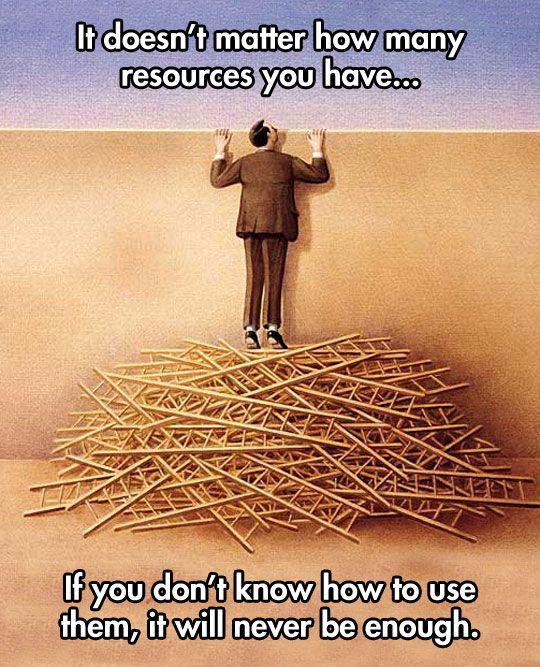
\includegraphics[width=0.6\textwidth]{images/chapter-03/resources-doesnt-matter.jpg}}

\par\medskip\ABNTEXfontereduzida\selectfont\textbf{Source:} Unknown authorship.%\citeauthor{manualufpe2020} (\citeyear{manualufpe2020}) \par\medskip
\end{figure}

Personal conversion factors "influence how a person can convert the characteristics of the commodity into a functioning" \cite[p.~99]{robeyns:2005}. I can list examples of these factors as metabolism (e.g., Do you have thyroid problems? Are you old or young?), physical condition (Are you tired? Are you disabled?), sex (e.g., Are you a woman? Are you a transgender?), reading skills (e.g., Do you know how to read? Do you know how to read English?), and intelligence (e.g., Are you competent at this? Do you have all the pre-requirements for it?). For instance, requesting \gls{CSE} students to do a reading task might not face any problem if they are well-nourished. but if they are not, we should ask ourselves what (and how) we may require of them, even knowing their food vulnerability, to respond to our requirements adequately.

Social conversion factors are directly related to the society in which people live. I can list as examples: public policies (e.g., affirmative actions, minimum income), social norms (e.g., "boys dress blue, girls dress pink", handshaking), discriminating practices (e.g., racism, homophobia), gender roles (e.g., "ladies first"), societal hierarchies (e.g., monarchy, patriarchalism), and power relations (e.g., professor-student, boss-employee). For instance, requesting \gls{CSE} students to do a reading task on Saturdays can face religious barriers. If you have one who is a member of the Seventh-day Adventist Church, this student can allegate impossibility to do this therefore Saturday is a holy day for them\footnote{By the way, I used "they/them" in this phrase to refer to someone that I do not know who is in relation to gender or sex orientation (see more in \url{https://www.npr.org/2021/06/02/996319297 /gender-identity-pronouns-expression-guide-lgbtq}). This is another example of social norm.}.

Lastly, environment conversion factors "emerge from the physical or built environment in which a person lives" \cite{robeyns:2023}. I can list as examples climate (e.g., arid, rainy), geographical location (e.g., rural, urban), proneness to natural disasters (e.g., earthquake, hurricane), and availability of natural resources (e.g., river, wood). Requesting \gls{CSE} students to go to the library to get a book immediately after a hurricane hit, for instance, can be unfeasible, and consequently, they would not have the capability for it.

I conclude this section with another \citeauthoronline{sen:1992} (\citeyear{sen:1992}, p.~38) assertion about conversion factors: 
\begin{citacao}
    "If we are interested in the freedom of choice, then we have to look at the choices that the person does in fact have, and we must not assume that the same results would be obtained by looking at the resources that he or she commands. The moves towards resource-based interpersonal comparisons in contemporary political philosophy (such as those of Rawls and Dworkin) can certainly be seen as taking us in the direction of paying attention to freedom, but the moves are substantially inadequate. In general, comparisons of resources and primary goods cannot serve as the basis for comparing freedoms".
\end{citacao}
Equality of opportunities involves resources, but not only. The \gls{CA} approach provides us with a possible common vocabulary to analyze equity issues from different theoretical standpoints. After this discussion, we can define equity as the equality of capabilities. The challenge is identifying the crucial capabilities in a \gls{CS} program and proposing policies to guarantee them.

\citeonline[p.~98]{robeyns:2005} schematizes the concepts presented here generally (Figure \ref{fig:robeyns-representation}) without educational concerns nor representing a minimal dynamic related to the flux from current to expected functionings. Bearing in mind that there is no consensus as to how methodologically operationalizing \gls{CA} constructs (e.g., \citeonline[p.~157]{comim:2008}, \citeonline[pp.~65-69]{hart:2012}), I created a minimal dynamic flux to guide an educational equity analysis from \gls{CA} lens (Figure \ref{fig:grouped-robeyns-representation}), indicating clearly three critical dimensions: Achievements (\acrshort{A}), \acrfull{M}, and Conversion Factors (\acrshort{CF}). 

\begin{figure}[ht!]
\centering

\caption{\textmd{A stylized non-dynamic representation of a person's capability set and her social and personal context.}}
\label{fig:robeyns-representation}
\fcolorbox{gray}{white}{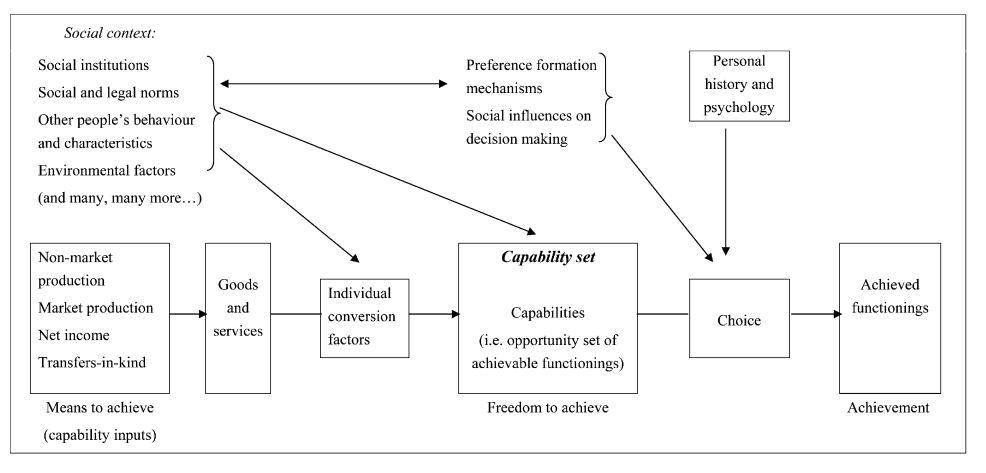
\includegraphics[width=0.9\textwidth]{images/chapter-03/robeyns-representation.png}}

\par\medskip\ABNTEXfontereduzida\selectfont\textbf{Source:} \citeonline[p.~98]{robeyns:2005}.
\end{figure}

\begin{figure}[ht!]
\centering

\caption{\textmd{A stylized dynamic representation of a student's capability set and their social and personal context.}}
\label{fig:grouped-robeyns-representation}
\fcolorbox{gray}{white}{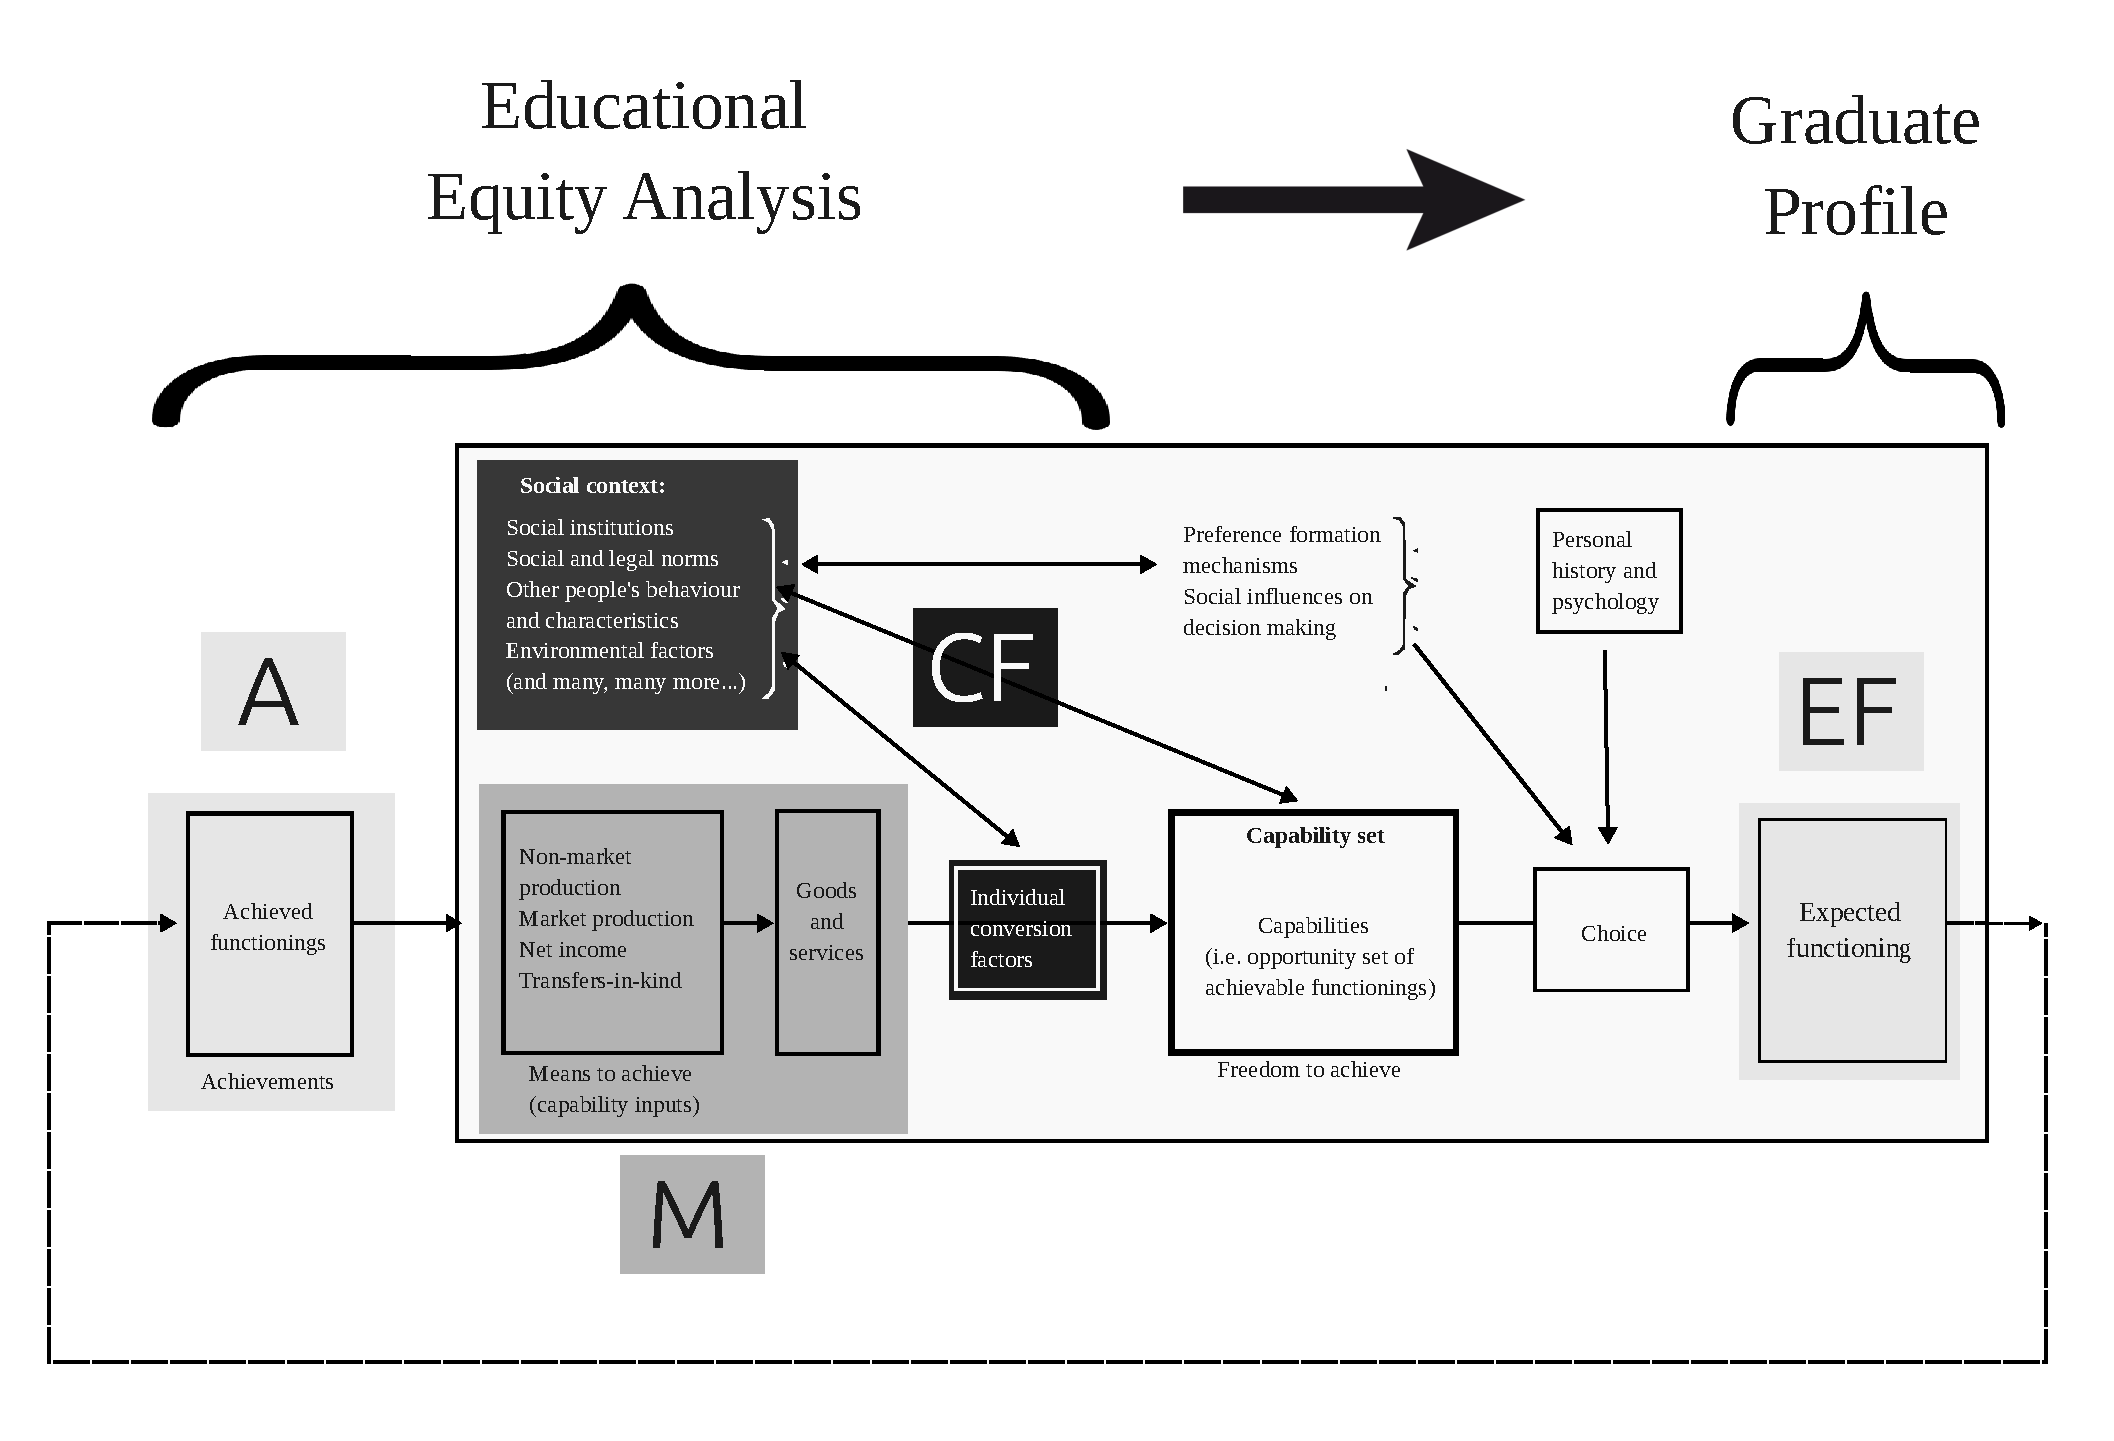
\includegraphics[width=0.9\textwidth]{images/chapter-03/grouped-robeyns-representation.pdf}}

\par\medskip\ABNTEXfontereduzida\selectfont\textbf{Source:} Created by the author (2024), adapted from \citeonline[p.~98]{robeyns:2005}.
\end{figure}

\subsection{Critiques to Capabilities Approach}
\label{sen-ss:critiques}

I can list at least two critiques to \gls{CA}. The first critique concerns the choice of a unifier lens. In the same way that Sen problematizes a resource-based lens, it is possible to extend his argument and assert that there is a level of arbitrariness in the choice of well-being as the unifier lens. Can we guarantee that this lens probably encompasses all dimensions of a complex equity analysis? Would this lens tend to value some aspects of an equity scenario more than others? Indeed, when we prefer one lens over another, our choice is carried by intentionality, and it is plausible to consider all implications of this decision. As this is a circular argument, anyone who advocates that their lens is preferable to another will be liable to suffer this kind of objection.

The second critique concerns the original \gls{CA} political standing. \gls{CA} is conceived under the liberal worldview, even situated closer to socio-liberalism. For this reason, \gls{CA} is reformist about how to proceed with the changes in our society and, consequently, not revolutionary (in a Marxist view). It is possible that some progressives or feminist researchers can not receive \gls{CA} gladly. For instance, \citeauthoronline{dejaeghere:2020} (\citeyear{dejaeghere:2020}, p.~17) approaches how postcolonial and feminist perspectives can be used to address critiques about the \gls{CA} related to questions of power and the individualized and decontextualized nature of capabilities. \gls{CA} research area is evolving the original Sen approach to appropriately consider these epistemological possibilities (e.g., critical capabilities \cite{walker:2010}).

When we presuppose a revolutionary perspective, it is essential to bear in mind the direct consequences of this choice. For instance, Figure \ref{fig:rliberation} presents a third frame proposing what should be a kind of liberation in the watching game scenario\footnote{Available by Center for Story-based Strategy (CSS) in: \url{https://www.storybasedstrategy.org/tools-and-resources}.}. The idea of providing the solution only by rearranging the box number available for each person can be read from a reformist perspective. We intervene in the box number but do not change the stadium structure, for example. The fence removal is concerned with modifying the structure at a higher level, aiming to solve this problem without recurring for a box redistribution. Although this action remedies the problem of watching games for those three people, it can generate other implicit problems that the stadium structure has already dealt with. Depending on the awareness level of the audience, the fence can play a collective role in preventing anyone from trespassing on the field and disturbing the expected flux of the game, affecting other people in the audience in their freedom to watch the game. It is totally plausible to shimmer possibilities to change the structure instead of providing only "make-up solutions" for equity problems. However, it is necessary to observe that some macro-structures in our society play multiple functions (primarily when we propose radical structural changes).

\begin{figure}[ht!]
\centering

\caption{\textmd{Illustration about the difference among equality, equity, and liberation.}}
\label{fig:rliberation}
\fcolorbox{gray}{white}{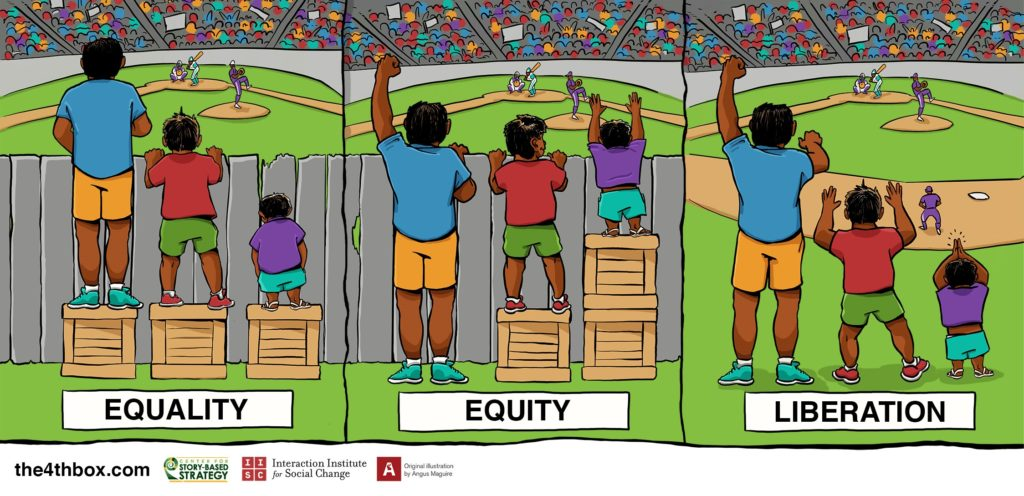
\includegraphics[width=0.9\textwidth]{images/chapter-03/liberation.jpg}}

\par\medskip\ABNTEXfontereduzida\selectfont\textbf{Source:} Unknown authorship.
\end{figure}

It is important to highlight that the reasons that I chose Rawls and Sen for this discussion in this research are (i) the agenda of social justice is not an exclusivity of progressive perspectives, and (ii) Sen contributes to this discussion from a differentiated place of speech; he is from the Global South and knows the hardness of social inequalities in his own country (India).
